% main.tex — Paper 2: la frontera de amortización de la memoria
% procedimental (outline: docs/paper2-honest-outline-2026-08-11.md).
%
% Venue DE TRABAJO: EMSE (mismo template svjour3 que el Paper 1; decisión
% formal la toma /paper-match con el manuscrito completo — S4). La clase
% y el .bst vienen copiados de paper/ (zip oficial Springer).
% Compilar: make  (o pdflatex main && bibtex main && pdflatex ×2)
%
% Estado S1 (2026-08-15): Results ESCRITO desde los datos cerrados
% (síntesis M1 + A/B project-memory), modelo de amortización escrito
% (corto y central), Methods/Intro/RW como esqueleto estructurado con
% fuentes. Los TODO marcan prosa por escribir. NO se corre ningún sweep
% nuevo para este paper (regla del outline § "Qué existe y qué NO").

\documentclass[smallcondensed,natbib]{svjour3}
\journalname{Empirical Software Engineering}

\usepackage[utf8]{inputenc}
\usepackage[T1]{fontenc}
\usepackage{graphicx}
\usepackage{booktabs}
\usepackage{amsmath}
\usepackage[colorlinks=true, linkcolor=blue, citecolor=blue, urlcolor=blue]{hyperref}
\usepackage{xcolor}

\newcommand{\braze}{\textsc{braze}}
\newcommand{\todo}[1]{\textcolor{red}{[TODO: #1]}}

\title{When Procedural Memory Does Not Pay: the Amortization Frontier
of Prompt-Injected Memory for Local-First Coding Agents%
\thanks{\todo{grants / acknowledgements}}}
\titlerunning{When Procedural Memory Does Not Pay}

\author{Francisco Parra}

\institute{F. Parra \at
  Departamento de Ingenier\'ia Inform\'atica, Universidad de Santiago de
  Chile, Santiago, Chile \\
  \email{francisco.parra.o@usach.cl}
}

\date{Received: date / Accepted: date}

\begin{document}
\maketitle

% =====================================================================
\begin{abstract}
% Fuente: docs/paper2-honest-outline-2026-08-11.md (§ claim + § por qué
% un nulo es publicable). Redactar al FINAL (S3), tras Results/Model.
\todo{Abstract (escribir al final). Espina: (1) distilling cloud-tutor
interventions into reusable procedural playbooks for local agents
``sounds obviously good''; (2) we formalize the amortization condition
such memory must satisfy and show, across two independent
pre-registered evaluations (140 runs; 306 runs), that prompt-injected
procedural memory falls on the wrong side of it precisely where it
would be needed; (3) a same-prompt control arm converted an apparently
significant $+13$-task gain ($p=0.011$, Holm-corrected) into an
unattributable $+4$ ($p=0.541$) --- without that arm the result would
have been published as a false positive; (4) design lesson: either
injection cost drops (retrieval-on-demand) or round savings rise
(class-unlocking interventions); both directions are measured, not
speculated.}
\keywords{agentic coding \and procedural memory \and small language
models \and negative results \and pre-registration \and same-prompt
control}
\end{abstract}

% =====================================================================
\section{Introduction}\label{sec:intro}
% Fuente: outline § "El giro" + § "Por qué un nulo es publicable".
% Anclas de urgencia para RW: CompInt (arXiv 2608.11242, pérdida de
% memoria/constraints en compactación), AutoDesign (arXiv 2608.13560,
% meta-harness con Context&Memory como componente), cola verify-refs.
\todo{Intro (S3). Puntos fijos del outline:
(1) memory-augmented agents: la técnica ``destila la intervención del
tutor cloud en un playbook local reutilizable'' es exactamente el tipo
de idea plausible que se adopta sin medir;
(2) claim central: la memoria procedimental inyectada por prompt tiene
una frontera de amortización estrecha y cuantificable, y la técnica
ingenua cae del lado equivocado de ella --- con una anti-correlación
entre cuándo ayuda (tareas ya memorizadas) y cuándo se necesita
(tareas frescas);
(3) contribuciones: (a) formalización de la condición de amortización;
(b) dos nulos independientes pre-registrados que la confirman, con el
control del mismo-prompt como instrumento metodológico transferible;
(c) el benchmark multi-sesión A$\to$B$\to$H; (d) la lección de diseño
con dirección medida (retrieval-on-demand o class-unlocking).}

% =====================================================================
\section{Background and Related Work}\label{sec:related}
% Cola bib: CompInt (compaction loss), AutoDesign (meta-harness),
% Paper 1 (self-cite braze), memoria agéntica (Voyager/Reflexion-style,
% skill libraries), + entradas ya en cola: zhu2026babeltele,
% walkinglabs2026, dex2026wsff, luo2026autodesign. /verify-refs en S4.
\todo{RW (S3): (a) memoria episódica/procedimental en agentes LLM
(skill libraries, reflection, playbooks); (b) agentes locales/SLM y el
costo real de los tokens de contexto en inferencia local; (c) pérdida
de memoria estructural en el harness (CompInt) y el harness como
objeto de optimización (AutoDesign, y la taxonomía de 5 componentes
donde Context\&Memory es uno); (d) resultados negativos y
pre-registro en ESE empírico.}

% =====================================================================
\section{The Amortization Condition}\label{sec:model}
% Fuente: outline § "El claim que los datos SÍ sostienen". Sección
% CENTRAL y corta — la fórmula que Results instancia.

Prompt-injected procedural memory --- a playbook, a list of files
touched in previous sessions, a distilled tutor intervention ---
enters the agent's context on \emph{every} round of a turn: agentic
loops re-send the (growing) conversation to the model each round, so a
memory section of $c$ tokens does not cost $c$ tokens per task but
$c \times R$ tokens, where $R$ is the number of rounds the turn takes.
Its benefit, in turn, is realized as \emph{rounds saved}: if the
memory actually guides the model, the turn converges earlier.

Let $R_{\mathrm{base}}$ and $T_{\mathrm{base}}$ be the mean rounds and
mean input tokens per round of the memory-free agent on a task, and
let $\Delta R = R_{\mathrm{base}} - R_{\mathrm{mem}}$ be the round
reduction the memory produces. Injection adds a per-round overhead
$\Delta T = T_{\mathrm{mem}} - T_{\mathrm{base}}$. The memory
\emph{amortizes} --- saves net input tokens --- if and only if

\begin{equation}\label{eq:amortization}
\underbrace{\Delta R \cdot T_{\mathrm{base}}}_{\text{rounds no longer
paid}} \;>\; \underbrace{\Delta T \cdot
R_{\mathrm{mem}}}_{\text{overhead on every surviving round}} .
\end{equation}

Equation~\eqref{eq:amortization} makes the trade explicit: a memory
section that costs a few hundred tokens per round must buy a
substantial fraction of a round to break even. For the configurations
measured in this paper ($T_{\mathrm{base}} \approx 1{,}400$ tokens per
round, $R_{\mathrm{mem}} \approx 6$ rounds, $\Delta T \approx
200$--$270$ tokens), the break-even round reduction is $\Delta R^{*} =
\Delta T \cdot R_{\mathrm{mem}} / T_{\mathrm{base}} \approx 0.9$--$1.2$
rounds --- the memory must eliminate about one full round of
interaction to pay for itself. The central empirical question is
whether realistic procedural memory clears that bar on the tasks where
it is actually needed. Our measurements
(Section~\ref{sec:results}) show that it clears it only on a task the
model already knows --- where the memory is redundant --- and misses
it by a factor of $3$--$6\times$ on fresh tasks --- where it would
matter. We refer to this as the \emph{anti-correlation} between when
memory helps and when it is needed.

% =====================================================================
\section{Method}\label{sec:method}
% Fuente: docs/project-memory-design.md, braze-memory (crate),
% docs/paper2-memory-distillation-protocol-2026-07-16.md (bench A→B→H),
% docs/hypothesis-2026-08-04-project-memory-ab.md (diseño A/B + gate).
\todo{Methods (S2). Subsecciones previstas:
\textbf{Harness e infraestructura}: \braze{} (self-cite Paper 1),
LearnedPlaybook tipado + lifecycle (candidate$\to$validated) +
schema, hook de ProjectMemory; ejecución local (gpt-oss:20b, Nitro,
LocalBackend/Harmony u Ollama según sweep — declarar por experimento).
\textbf{Estudio 1 (M1)}: benchmark multi-sesión A$\to$B$\to$H
(sesión A genera el playbook con tutor; tareas B miden transferencia
dentro de la familia \texttt{rust\_compile\_repair}; H holdout);
brazos none vs human-playbook (el más fuerte a priori: escrito por
humano, no destilado), n=20 por celda, 3 pares B + holdout = 140
corridas, seeds 42--61, mismo backend.
\textbf{Estudio 2 (project-memory A/B)}: los tres brazos
(baseline / hook-con-memoria-vacía / hook-seeded), suite
discriminante de 34 tareas con oráculo \texttt{cargo check}, 3
repeticiones, 306 corridas; el brazo vacío como \emph{same-prompt
control} (prompt idéntico al baseline por construcción); gate de
plomería pre-registrado; McNemar exacto pareado + Holm.
\textbf{Pre-registro}: ambos estudios con hipótesis, criterios de
decisión y prior honesto commiteados antes de correr (git-only
registration); citar los dos docs con hash.}

% =====================================================================
\section{Results}\label{sec:results}
% Fuente tablas: docs/sweep-memory-distillation-3taskB-synthesis-
% 2026-07-17.md (JSON: docs/sweep-memory-distillation-r20-moveB-
% 2026-07-17.json, 140 corridas) y docs/hypothesis-2026-08-04-
% project-memory-ab.md § Resultados finales (JSONs: docs/pm-ab/).

\subsection{Study 1: a human-written playbook pays only where it is
redundant}\label{sec:results-m1}

Table~\ref{tab:m1} shows the three task pairs of the M1 pilot: the
same human-written playbook --- the strongest memory variant a priori,
authored by a human rather than distilled by a model --- attached to
three compile-repair tasks of the same family
(\texttt{rust\_compile\_repair}), $n=20$ per cell, identical seeds and
backend across arms.

\begin{table}
\caption{Study 1 (pilot M1): the same human playbook on three tasks of
the same family ($n=20$ per cell, gpt-oss:20b, seeds 42--61).
$\Delta R$ = mean rounds saved by the playbook; net $\Delta$tokens =
mean input tokens (playbook) $-$ mean input tokens (none), negative =
the playbook saves net tokens. Only the task the model already knows
amortizes.}
\label{tab:m1}
\begin{tabular}{lcccccc}
\toprule
Task & Pass (none$\to$pb) & Rounds (none$\to$pb) & $\Delta R$ &
Tok/round (none$\to$pb) & Net $\Delta$tokens & Wall s (none$\to$pb) \\
\midrule
\textsc{original} (saturated) & 14/20$\to$16/20 & 6.70$\to$5.75 &
$\mathbf{+0.95}$ & 1406$\to$1590 & $\mathbf{-304}$ &
57.4$\to$40.6 ($p=0.003$) \\
\textsc{loop} (E0502, fresh) & 15/20$\to$14/20 & 5.60$\to$5.45 &
$+0.15$ & 1383$\to$1625 & $+1076$ & 49.5$\to$51.2 ($p=0.55$) \\
\textsc{move} (E0382, fresh) & 18/20$\to$15/20 & 6.40$\to$6.05 &
$+0.35$ ($p=0.035$) & 1394$\to$1662 & $+1132$ & 48.5$\to$47.0
($p=0.62$) \\
\bottomrule
\end{tabular}
\end{table}

The pattern instantiates Equation~\eqref{eq:amortization} exactly. On
the \textsc{original} task --- the canonical bug the model already has
memorized, where it passes without help --- the playbook saves nearly
a full round ($\Delta R = 0.95$, right at the $\Delta R^{*} \approx
0.9$--$1.2$ break-even), and the net token balance is negative
($-304$): the memory amortizes. On the two fresh tasks, the round
reduction collapses to $+0.15$ and $+0.35$ --- a factor of $3$--$6$
below break-even --- while the per-round overhead stays fixed at
$+243$ and $+268$ tokens, so the playbook \emph{costs} $+1076$ and
$+1132$ net tokens per task. Figure~\ref{fig:frontier} places the
three tasks against the amortization frontier.

Pass rate shows no consistent signal in any pair (Fisher $p=0.72$,
$1.00$, $0.41$), and the point direction is \emph{negative} in two of
three ($15\!\to\!14$, $18\!\to\!15$), positive only on the saturated
task. There is no evidence, in any of the three pilots, that this
playbook reliably improves success --- the efficiency gain on the
saturated task is the only positive result of the entire pilot, and it
does not generalize even within the same bug family.

\begin{figure}
\centering
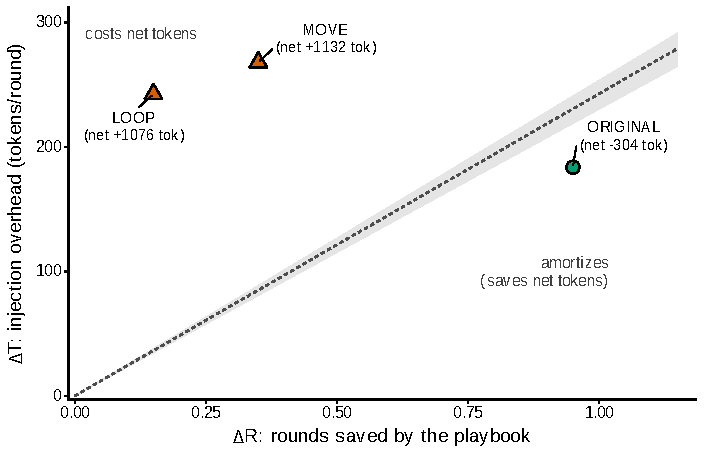
\includegraphics[width=\textwidth]{figs/fig1_frontera.pdf}
\caption{The amortization frontier (Eq.~\ref{eq:amortization}) on the $(\Delta R, \Delta T)$ plane, with the three task pairs of Study 1 ($n=20$ per cell) computed from the committed raw runs. The shaded band spans the per-task break-even curves $\Delta T^{*} = \Delta R \cdot T_{\mathrm{base}} / R_{\mathrm{mem}}$. Only the task the model already has memorized (\textsc{original}, circle, net $-304$ tokens) falls on the amortizing side; the two fresh tasks (triangles) sit $3$--$6\times$ above their break-even, costing $+1076$ and $+1132$ net tokens per task.}

\label{fig:frontier}
\end{figure}

\subsection{Study 2: the same-prompt control removes the headline
effect}\label{sec:results-pm}

The second study evaluates the harness-integrated form of the same
idea: a project-memory hook that injects, into the system prompt, the
files touched in previous sessions. Because the benchmark opens a
fresh session per repetition, the plain hook arm runs with empty
memory and renders \emph{nothing} --- its prompt is identical to the
baseline by construction. That accident of plumbing is
methodologically precious: the empty arm is a \textbf{same-prompt
control}, and any paired discordance between it and the baseline is an
in-sweep measurement of the noise floor. A third arm
(\emph{seeded}) synthesizes the memory a previous session would have
left, with zero experimenter-authored content.

\begin{table}
\caption{Study 2: \texttt{enable\_project\_memory} A/B on the
34-task discriminating suite, 3 repetitions per arm (306 runs,
gpt-oss:20b, LocalBackend/Harmony). The empty arm's prompt is
byte-identical to baseline (verified on preserved sessions, not
assumed).}
\label{tab:pm}
\begin{tabular}{lccc}
\toprule
Arm & Pass & Mean input tokens & Mean rounds \\
\midrule
baseline & 59/102 (57.8\%) & 13{,}526 & 5.5 \\
empty (same-prompt control) & 68/102 (66.7\%) & 18{,}709 & 6.7 \\
seeded & 72/102 (70.6\%) & 17{,}559 & 6.1 \\
\midrule
\multicolumn{4}{l}{seeded $-$ baseline: $+13$, McNemar exact
$p=0.011$ (Holm $0.021$)} \\
\multicolumn{4}{l}{empty $-$ baseline: $+9$, $p=0.078$} \\
\multicolumn{4}{l}{\textbf{seeded $-$ empty: $+4$, $p=0.541$}} \\
\bottomrule
\end{tabular}
\end{table}

Read without the control arm, Table~\ref{tab:pm} is a publishable
positive: seeded beats baseline by $+13$ tasks with a Holm-corrected
$p=0.021$, meeting the pre-registered promotion criterion \emph{in its
letter}. The control arm invalidates the premise: with a
byte-identical prompt, the empty arm rose $+9$ on its own, and the
only contrast that isolates the \emph{content} of the memory ---
seeded vs.\ empty --- is null ($+4$, $p=0.541$). Attributing the
headline to the memory would have been exactly the error the control
arm existed to prevent. The lever was not promoted.

The pre-registered plumbing gate fired first: baseline vs.\ empty
showed 21 paired discordant cells against a pre-registered threshold
of $\leq 2$. The diagnostic (preserved sessions on the four most
discordant tasks) established that (i) round-1 prompts were
token-identical across arms in all 12 pairs --- proven, not assumed;
(ii) no trajectory ever observed the hook's on-disk state; and (iii)
a re-run inverted the direction of the discordances. Verdict: the 21
discordances were noise. The collateral finding is itself a result:
\textbf{the noise floor is configuration-specific} --- the $\leq 2$
threshold, borrowed from the floor measured on an easier suite,
underestimated the discriminating-suite floor by an order of magnitude
($\sim$20\% of cells flip under identical prompts at temperature 0.2).
Every future A/B in this regime needs an in-sweep same-prompt control
rather than a floor imported from another configuration.

\subsection{Cost of the injected section}
% Fuente: hypothesis-2026-08-04 § Decisión (costo ~40 tokens ronda 1) y
% síntesis M1 (200-270 tokens/ronda del playbook).
The two studies bracket the injection-cost regime that
Equation~\eqref{eq:amortization} prices. The M1 playbook adds
$\sim$200--270 tokens \emph{per round} (a methodology section the
designer consults every round); the project-memory section is small
($\sim$40 tokens in round 1) but correspondingly carries no measurable
content signal. Between them: an injection cheap enough to be
harmless was too thin to matter, and an injection rich enough to
matter was too expensive to amortize on fresh tasks. The frontier is
narrow from both sides.

% =====================================================================
\section{Discussion}\label{sec:discussion}
% Fuente: outline § contribución 4 + § threats.
\todo{Discussion (S2/S3):
(1) la anti-correlación como el hallazgo con dientes: la memoria ayuda
donde es redundante y no ayuda donde haría falta;
(2) por qué el nulo importa: la técnica ``suena obviamente buena'' y la
comunidad la adoptaría sin medir; disciplina de nulos del proyecto
(citar Paper 1: edit-fence vs evidencia aider, TTC, etc.);
(3) el control del mismo-prompt como instrumento transferible: sin él,
este paper reportaría un $+13$ significativo falso;
(4) direcciones con perfil de costo distinto (future work medido, no
especulación): (a) memoria FUERA del prompt recuperada bajo demanda
(perfil AGENTS.md-JIT: costo solo cuando se usa); (b) intervenciones
que desbloquean una CLASE de tarea (round savings grandes);
(c) frontera sesión-vs-proyecto: session constraints como caso límite
de memoria durable (SC-retention, si el sweep corre antes del freeze:
sección corta; si no, forward reference honesta);
(5) relación con CompInt (la compactación PIERDE memoria — nosotros
medimos que inyectarla tampoco es gratis: las dos mitades del mismo
presupuesto de contexto) y con AutoDesign (Context\&Memory como
componente optimizable: nuestra ec.~\ref{eq:amortization} es el
criterio de aceptación que ese componente necesita).}

% =====================================================================
\section{Threats to Validity}\label{sec:threats}
% Fuente: outline § threats — casi redactado ahí; expandir en S3.
\todo{Threats (S3, espina del outline):
(1) una sola familia de tareas (\texttt{rust\_compile\_repair}) — la
frontera podría moverse donde la intervención desbloquea más rondas;
(2) un solo modelo (gpt-oss:20b) — el balance $\Delta T / \Delta R$
depende del modelo; uno más débil tiene más margen de rondas que
recuperar (direccional, no medido);
(3) el nulo es de la memoria EN EL PROMPT — retrieval-on-demand tiene
otro perfil de costo (es la contribución 4, no una amenaza);
(4) variantes summary/procedural/lead-fallback del protocolo original
sin pilotear — pero todas agregan MÁS costo de inyección que el
human-playbook ya negativo: predicción declarada, no medición;
(5) Ollama no bit-exacto con seed fijo (efectos secundarios de wall
time inestables entre corridas; el efecto primario de tokens replica).}

% =====================================================================
\section{Conclusion}\label{sec:conclusion}
\todo{Conclusion (S3). Una técnica obviamente buena, medida con
pre-registro y controles, no paga donde se la necesita; la condición
de amortización dice exactamente qué tendría que cambiar para que
pague. Ambas salidas (bajar costo de inyección, subir ahorro de
rondas) quedan medidas como dirección.}

% =====================================================================
% Declaraciones EMSE (rellenar en S4 con /paper-submit)
\begin{acknowledgements}
\todo{acknowledgements}
\end{acknowledgements}

\section*{Declarations}
\todo{Data availability (repo + JSONs commiteados + tag), conflicts,
CRediT, uso de IA — mismas plantillas que el Paper 1.}

% =====================================================================
\bibliographystyle{spbasic}
% \bibliography{refs}  % refs.bib en S3 (cola: CompInt, AutoDesign,
% Paper 1, memoria agéntica, zhu2026babeltele, walkinglabs2026,
% dex2026wsff, luo2026autodesign — /verify-refs en S4)

\end{document}
